\documentclass[hidelinks,12pt]{article}
\usepackage[utf8]{inputenc}
\usepackage{parskip}
\usepackage[UKenglish]{babel}
\usepackage[headheight=15pt,margin=3cm]{geometry}
\usepackage{multirow}
\usepackage{multicol}
\usepackage[colorlinks=false]{hyperref}
\usepackage[super,square]{natbib}
\usepackage{float}
\usepackage[toc,page]{appendix}
\usepackage[table]{xcolor}
\usepackage{titling}
\usepackage{array}

\usepackage{color}
\usepackage{listings}
\usepackage{graphicx}
\usepackage{caption}
\usepackage{wrapfig}
\usepackage{lscape}
\usepackage{rotating}
\usepackage{epstopdf}
\usepackage{pifont}
\usepackage{gensymb}

\setlength{\parindent}{2em}

\date{March 2017}
\title{Music Performance Analysis Systems\\\large{Reference Guide}}
%\title{Systems Programming for Arm\\ DocetOS Assignment Technical Report}
\author{Y0070832}

\begin{document}
\maketitle
\tableofcontents
\newpage
\section{Executive Summary}
This reference guide provides information about the `\textit{PyTempo}' tempo-detection and active-metronome performance analysis system, including details of the implementation and underlying theory, as well as notes on using the software. \textit{Pytempo} provides a musician with access to two different functionalities designed to be useful whilst practising their instrument. Firstly the system analyses the sound of their performance and attempts to detect the tempo. This helps performers learn and practice playing at a specific tempo whilst unaccompanied. The second function is an active-metronome system, whereby a user can select a tempo and the system will supply a metronome at this tempo, whilst also detecting beats in the users performance and providing a visual comparison of the accuracy of these in relation to the metronome.

The system is implemented as a single piece of software in the python programming language, and utilises the PyAudio audio processing framework for the real time audio requirements, as well as the PyQt graphical user interface framework. Both are freely available to use for non-commercial products, and are used within the constraints of fair-use.
\section{Signal Processing Theory} \label{Processing}
The key elements of signal processing underlying this system are beat detection and tempo calculation. \textit{PyTempo} is a digital audio system, hence the processing is done in the digital domain, and the results are achieved using relatively simple techniques.
\subsection{Beat Detection} \label{BeatDetection}
Detecting beats in a digital audio signal can be achieved by looking for peaks in the energy waveform of the signal. A digital audio signal is comprised of a large number of individual samples, which are grouped into chunks. An energy value for each chunk can be calculated by taking the square of each of the samples in the chunk and summing them all together. For a stereo signal the value of both channels can be included, as shown in equation \ref{eq:EnergySum}

\begin{equation} \label{eq:EnergySum}
	E_i = \sum_{i=1}^{M}(left[i]^2 + right[i]^2)
\end{equation}

In order to detect peaks the system must compare the energy value of the most recent chunk to the average energy value over some window. In order to do this the previous energy values for a number of chunks are stored in a queue. A 1 second window is often a good size, and at a sample rate of 44.1 kHz this requires around 43 energy values to be stored. When a new chunk of samples arrives, the energy value is calculated and compared to the average energy value of the queue. If the new value exceeds the average by some threshold factor, a peak is detected in that chunk. For the purposes of this system, a peak indicates a beat.

\begin{equation}
	E > T\Bigg(\frac{1}{N}\sum_{i=1}^{N}E_i\Bigg)
\end{equation}

In order to give the best chance of accurately detecting the peaks, the threshold value must vary over time depending on the energy content of the signal. In order to do this the threshold is linked to the variance of the energy waveform by a linear regression.

\subsection{Tempo Detection}
The first of PyTempo's two operating modes attempts to calculate a local tempo value for what the performer is currently playing. To do this using the peak/beat detection method outlined in section  \ref{BeatDetection} the software must compare the intervals between subsequent detected beats. First an average of the inter-beat intervals is acquired using equation \ref{eq:IntervalAverage},

\begin{equation} \label{eq:IntervalAverage}
	I_{avg} = \frac{1}{N}\sum_{i=2}^{N}(t_i - t_{i-1})
\end{equation}

where $N$ is the total number of detected beats and $t_i$ is the time of detected beat $i$. Then a local tempo is calculated from this average using equation \ref{eq:Tempo},

\begin{equation} \label{eq:Tempo}
	T_{local} = \frac{60}{(I_{avg} / F_s)}
\end{equation}

where $I_{avg}$ is the average interval calculated before and $F_s$ is the sample rate. Note that using the beat detection method outlined in section \ref{BeatDetection} will give the beat times in terms of chunks, not individual samples as required by equation \ref{eq:IntervalAverage}, so the system must first multiply through by the chunk size to achieve a meaningful result.
\section{Performance Analysis System - PyTempo} \label{PyTempo}
\subsection{User Interface}
Both of PyTempo's modes feature graphical user interfaces and real time feedback, in a minimilast, bold visual style.
\subsubsection{Tempo Detection Mode}
Figure \ref{fig:TempoDetectScreenshot} shows the user interface for the tempo detection mode. The key features are the large numerical display for the estimated local tempo on the right, and a representation of the energy waveform on the left, where each bar indicates the energy of a single chunk. Chunks where a beat has been detected are highlighted in red. Both elements update in real time, with the waveform scrolling as new chunks are processed.

\begin{figure}[H]
	\begin{center}
		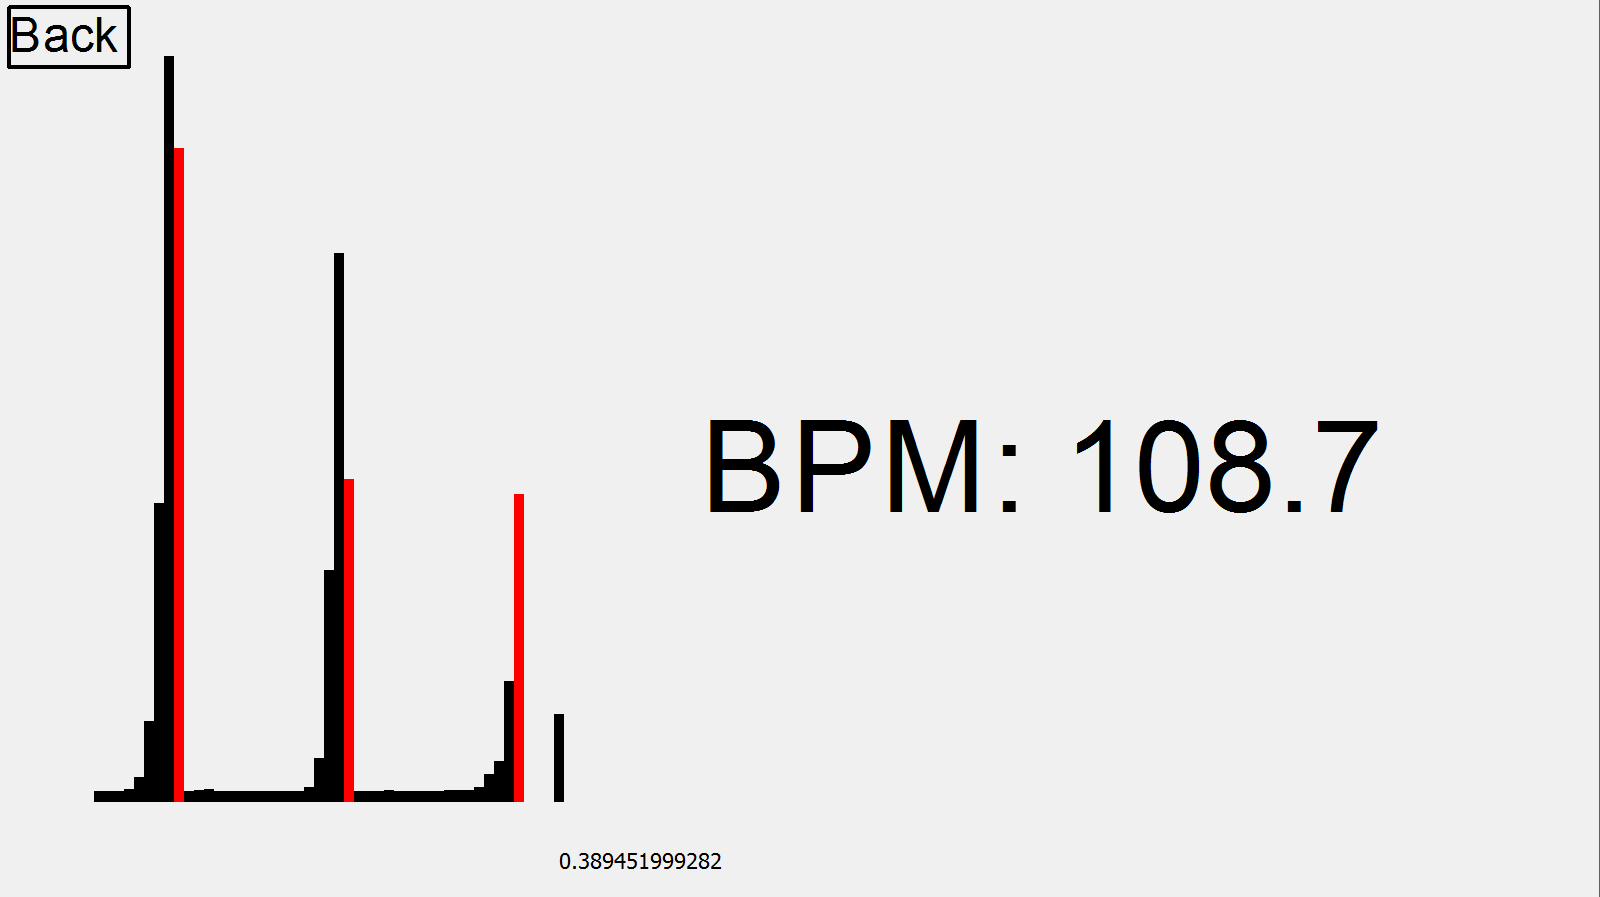
\includegraphics[scale=0.2]{TempoDetectScreenshot.png}
		\caption{Tempo detection mode interface}
		\label{fig:TempoDetectScreenshot}
	\end{center}
\end{figure}

\subsubsection{Active Metronome Mode}
Figure \ref{fig:ActiveMetronomeScreenshot} shows the user interface for the active metronome mode. The main feature of this interface is the graphical metronome timeline in the lower portion of the screen. The two horizontal lines form the timeline, and the dotted vertical line indicates the current instant. Metronome clicks are indicated by vertical lines beneath the timeline, and scroll from right to left, crossing the dotted line in time with the metronome clicks. The BPM controls in the top right hand corner allow the user to set their target tempo.

\begin{figure}[H]
	\begin{center}
		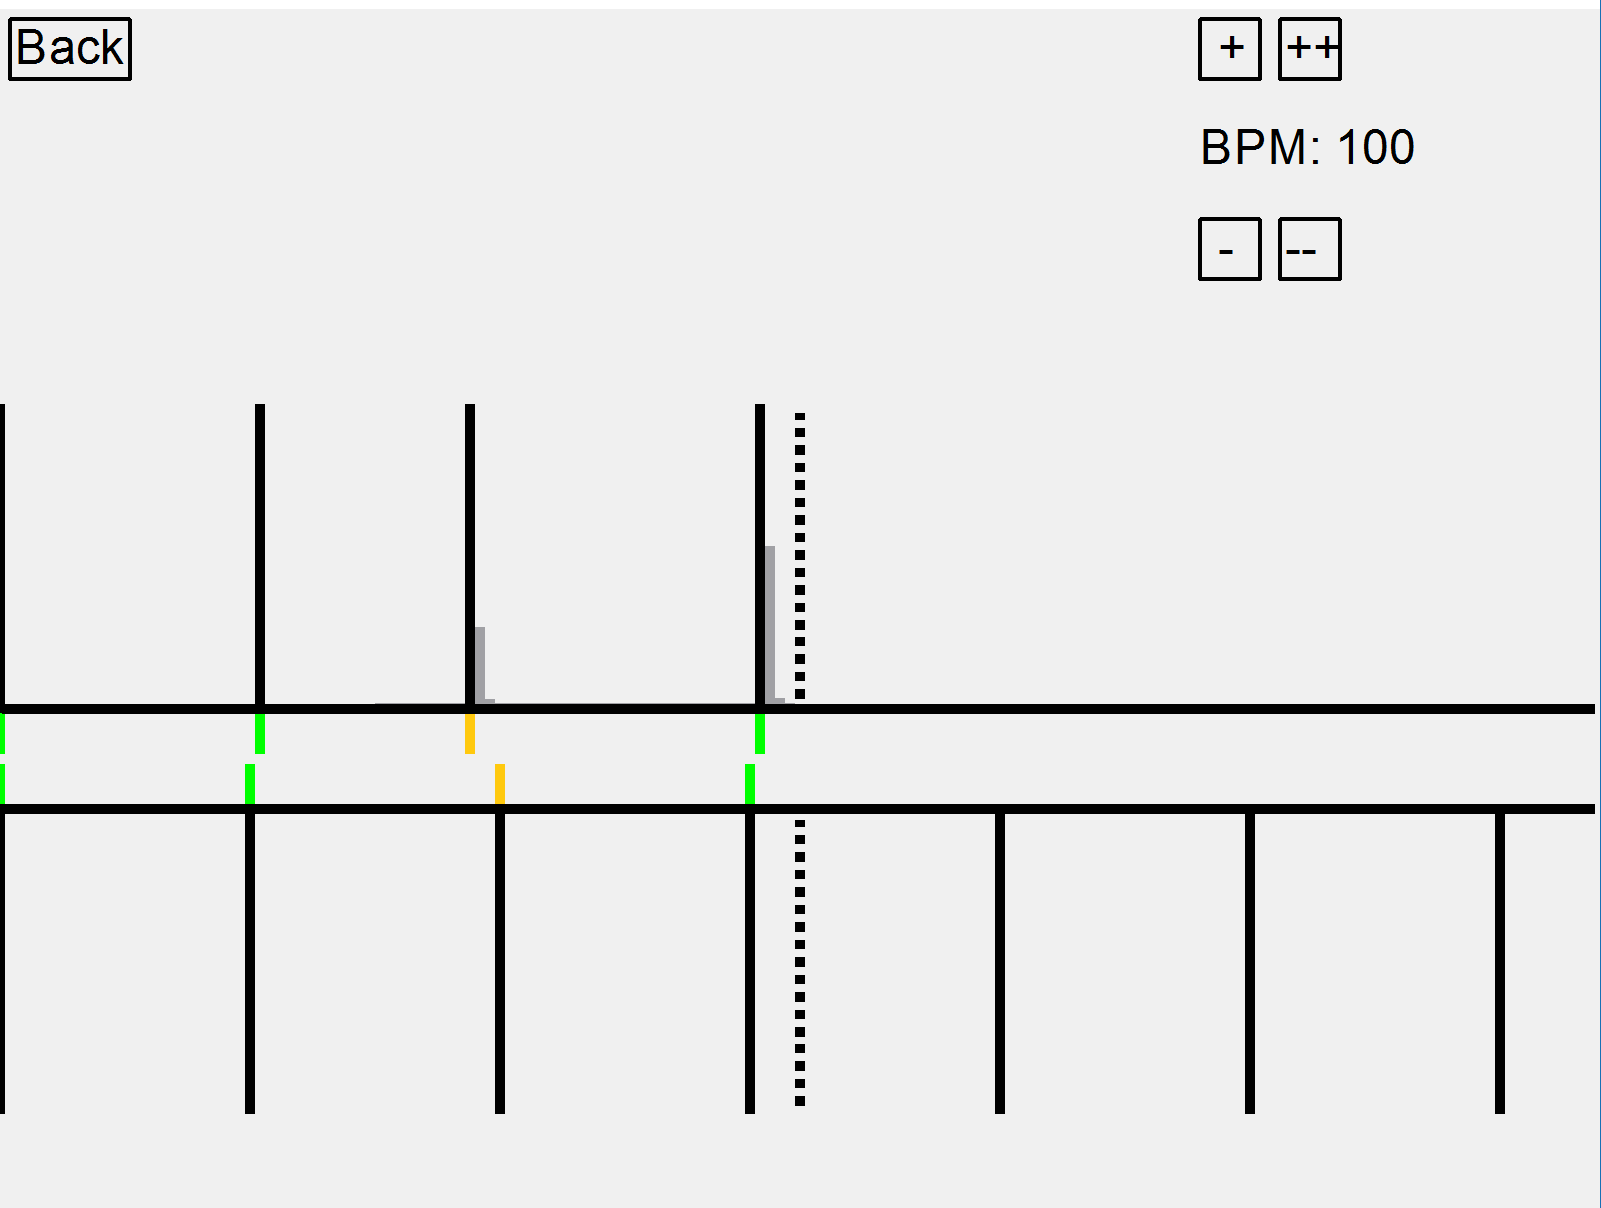
\includegraphics[scale=0.5]{ActiveMetronomeScreenshot.png}
		\caption{Active metronome interface}
		\label{fig:ActiveMetronomeScreenshot}
	\end{center}
\end{figure}


\subsection{Code Structure}
The software is organised into a number \textit{.py} code files, organised logically according to object-oriented programming (OOP) practices wherever possible. One extra file, `\textit{MetroClick.wav}' is provided along with the code, and contains the metronome sound. The main file is \textit{MPAS.py}, containing the entry point for the application. \textit{audioHandler.py} contains the code related to managing the PyAudio streams and other audio processing routines such as peak detection. The remaining files encapsulate individual elements of the programming, including the active metronome data in \textit{activeMetronome.py}, the routines for drawing the different UIs on the screen in \textit{renderer.py} and an encapsulation of a button component in \textit{button.py}.

\subsection{Running the Software}
\textit{PyTempo} can be run from the command line using Python 2.7, provided that the PyAudio and PyQt packages are installed. \textit{PyTempo} is also provided as a compiled binary executable for Windows, and can be run in this format without the PyAudio or PyQt frameworks available.

\section{System Evaluation and Future Work}
This guide accompanies the first version of PyTempo, which makes good headway in trying to achieve the system's aims. However a number of improvements could be made for future versions. The peak detection method is effective, however some more complex, higher level processing of the detected peaks could help to better detect tempo from more complex and less regular rhythms. Some pre-processing could also be applied to separate the incoming audio into grouped frequency components and isolate elements important to the beat, perhaps based on a target instrument selected by the user. The tempo estimation could potentially be improved through the use of a more in-depth averaging technique such as Kalman filtering.

\end{document}
